\subsubsection{FAST FPGA implementācijas modelis} \label{sec:fast-fpga}
FAST potenciālās ātrdarbības salīdzināšanai FPGA platformai, autors
izstrādājis savu implementācijas modeli. Pēc vairākiem uzbūves variantiem,
%TODO?: Atmestie modeļi?
autors par piemērotāko atzinis modeli, kas balstās uz atsevišķu apstrādes
vienību izmantoto resursu samazināšanu, un caurlaidspējas palielināšanu
instancējot lielu skaitu šo vienību.

Tā kā viena elementa --- punkta $\vec{p}$ piederības $F_9(\vb{I},t)$ ---
noteikšanas latentums nav prioritāte, apstrādes vienība, kā ilustrēts
\ref{fig:fast-fpga}~attēlā, resursu ekonomijas nolūkos, ir secīgas uzbūves.
Salīdzināšana ar apkārtnes punktiem notiek secīgi, to intensitātes vērtības
pārvietojot caur bīdes reģistru un ar skaitītājiem uzskaitot secīgu
gaišo un tumšo loka punktu skaitu. Šāda FAST-9 apstrādes vienība vienu punktu
var klasificēt $16+(n-1)=24$ takts ciklos, bet papildus takts cikli
var būt nepieciešami datu sagatavošanai.

\begin{figure}[tbh]
	\centering
	\def\svgwidth{\linewidth}
	{\small\input{img/fpga-model.pdf_tex}}
	\caption{Vienkāršota uzbūves shēma viena punkta apstrādes vienībai.}
	\label{fig:fast-fpga}
\end{figure}

Katra FAST punkta apstrādes vienība tad var tikt instancēta un vairāki
punkti klasificēti paralēli. Testiem tika izveidots
,,attēlu apgabalu procesors'', kas vienlaikus apstrādā $w \times w$ attēla
apakškopu, kur ${(w-6)}^2$ punkta apstrādes instances klasificē attēla
apakškopas punktus. Sintēzes rezultāti uzrādīja CPU līdzvērtīgu ātrdarbību
izmantojot tikai 18\% Virtex-6 resursu
(sk.~pielikumu~\ref{appx:test3}).

Lai arī ,,attēla apgabalu procesors'' ir adekvāta konstrukcija
ātrdarbības pārbaudei, tika konstatēts, ka lielāku attēlu dalīšana
apstrādei gabalos, ļoti neefektīvi izmanto pieejamo caurlaidspēju, ja
netiek izmantoti atmiņas buferi pārklājošās informācijas saglabāšanai.
Caurlaidspējas \newTerm{virstēriņa} (\termEn{overhead}) apjoms ir atkarīgs no
izvēlētā $w$ --- virstēriņš strauji samazinās pie lielāka $w$,
kā redzams \ref{fig:overhead}~attēlā, kur ar melnu, pārtrauktu līniju
atzīmēta nepieciešamā caurlaidspēja konstantai (patvaļīgi uzdotai)
mērķa veiktspējai.
\begin{figure}[tbh]
	\centering
	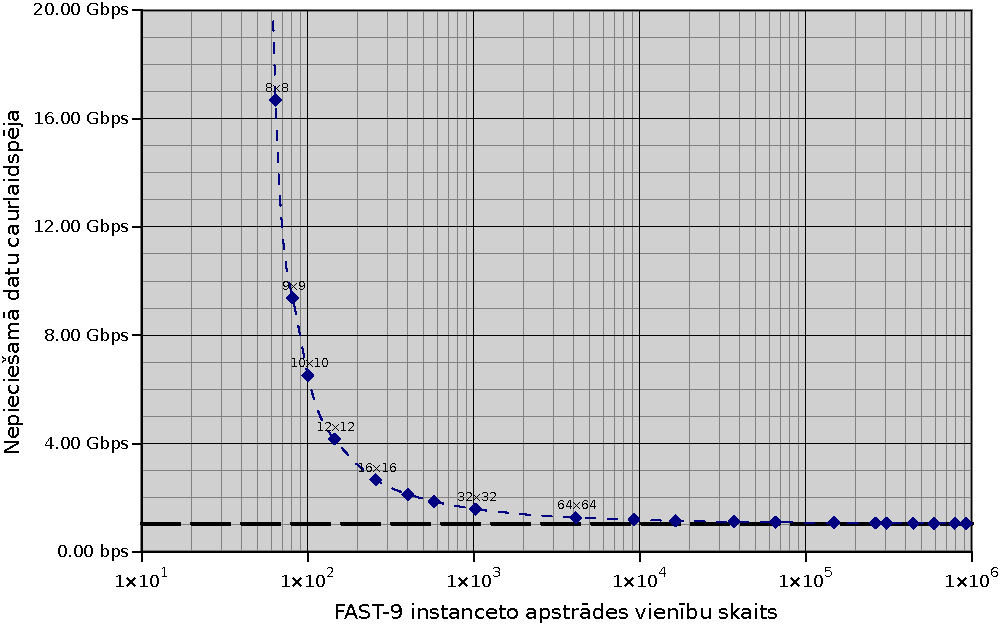
\includegraphics[scale=0.77]{chart-overhead}
	\caption{Caurlaidspējas virstēriņš pret FAST instanču skaitu.}
	\label{fig:overhead}
\end{figure}

Virstēriņš rodas, jo daļa no apstrādājamā attēla gabala, t.i.~tā malas,
satur nepilnīgu informāciju par punkta apkārtni. Tādēļ, lai apstrādātu
visu attēlu, apstrādes gabaliem ir jāpārklājas, kā ilustrēts
\ref{fig:chunks}~attēlā. Pie lielāka gabala malas garuma $w$,
virstēriņš mazinās.
\begin{figure}[tbh]
	\centering
	\def\svgwidth{0.9\linewidth}
	{\small\input{img/chunk-overhead.pdf_tex}}
	\caption{Apstrādājamais gabals un blakusesošo gabalu pārklāšanās.}
	\label{fig:chunks}
\end{figure}

Vienkāršākais risinājums būtu pārraidīt visu attēlu FPGA lokālā atmiņā,
un tad apstrādāt attēlu pa gabaliem, līdzīgi kā iepriekš. Šim
risinājumam ir divas problēmas: pirmkārt, FPGA atmiņas resursi bieži
vien ir ierobežoti, tādēļ visu attēlu var arī nebūt iespējams saglabāt,
pie tam papildus problēmas var sagādāt, ja attēla izmērs drīkst mainīties.
Otrkārt, atmiņas datu caurlaidspēja var papildus ierobežot
maksimālo $w$.

Par paraugu izmantotajam Virtex-6 (\texttt{XC6VLX75T}) FPGA,
ir 156 vienlaicīgi adresējami RAM bloki, ar
64 bitu maksimālo datu platumu (72 biti, ja izmanto 9.~baita bitu)%
\cite{Virtex6}. Maksimālā caurlaidspēja ir $156 \cdot \frac{64}{8} = 1248$
baitu takts ciklā, kas spēj nodrošināt
$\left\lfloor \frac{1248}{17} \right\rfloor = 73$ FAST punktu apstrādes vienības,
kas atbilst $8 \times 8$ apgabalam.
Ņemot vērā, ka apstrāde notiek vairākos takts ciklos, papildus
FAST vienības var tikt nodrošinātas ar datiem izveidojot datu
konveijeru (\termEn{pipeline}) līdz pat 24 pakāpēm
(kam gan trūkst loģikas bloku resursu izmantotajam FPGA).

Gadījumā, ja nav pieejami resursi visa attēla saglabāšanai atmiņā,
autors iesaka attēla dalīšanu gabalos divos līmeņos, t.i.~pārraides
vienībās, kas ir pietiekami lielas, lai mazinātu pārraides caurlaidspējas
virstēriņu, un apstrādes gabalos, kas pa daļām apstrādā lokālā atmiņā
uzglabātu pārraides vienību. Šādi tiek samazināts virstēriņš un var tikt
samazināts loģikas resursu patēriņš instancējot tikai tik FAST punktu 
apstrādes vienības, lai sasniegtu mērķa veiktspēju.

